\documentclass[fleqn,10pt]{wlscirep}
\usepackage[utf8]{inputenc}
\usepackage[T1]{fontenc}
\usepackage{float}
\usepackage{placeins}
\usepackage{multirow}
\usepackage{bm}
\usepackage{lineno}

\newcommand{\R}{\mathbb{R}}
\graphicspath{{figs/}}

\title{An Adaptive Graph-Fusion Extension to Conditional Local Convolution for Short-Range WeatherBench Forecasting}

\author[1,*]{Xinchen Geng}
\author[1]{Hung-Yu Lin}
\affil[1]{University of Southern California, Los Angeles, CA 90089, USA}
\affil[*]{gengx@usc.edu}

\keywords{Weather forecasting; Spatio-temporal graph neural networks; Adaptive graph learning; Spherical grids; Reproducibility}

\begin{abstract}
Conditional Local Convolution Recurrent Network (CLCRN) is an established
graph-recurrent model for meteorological forecasting. We examine whether a
compact adaptive graph-fusion (AGF) encoder can improve CLCRN by learning
non-local node dependencies before the original recurrent backbone. The
extension constructs a directed top-$k$ graph from trainable source and
destination node embeddings and combines graph-mixed and residual features
through a learned gate. Experiments use the WeatherBench preprocessing and
four tasks from the original CLCRN study: 2-m temperature, relative humidity,
10-m surface wind, and total cloud cover. We compare CLCRN-AGF with a
schedule-matched CLCRN control over five seed replicates. The clearest
effect is relative humidity: CLCRN-AGF reduces mean absolute error by 2.28\%
and root mean squared error by 3.02\%; all seeds improve (Welch tests:
$p=7.6\times10^{-4}$ and $p=8.4\times10^{-5}$). Effects on
temperature, wind, and cloud cover are small or metric-dependent. Component
ablations show that the adaptive graph branch contributes most clearly for
humidity, whereas replacing the learned gate by mean fusion remains
competitive. These results narrow the contribution of adaptive graph fusion:
it is useful for the humidity task but is not a uniformly beneficial
replacement for the original CLCRN encoder.
\end{abstract}

\begin{document}
\flushbottom
\maketitle
\thispagestyle{empty}
\linenumbers

\section*{Introduction}

Numerical weather prediction remains the operational standard because it
encodes atmospheric physics~\cite{bauer2015quiet}, while data-driven models
provide increasingly capable alternatives for selected forecasting tasks.
WeatherBench established a common ERA5-based benchmark for evaluating such
models~\cite{rasp2020weatherbench}. At the large-model end of the spectrum,
FourCastNet, Pangu-Weather, and GraphCast demonstrate the potential of neural
forecasting at global scale~\cite{pathak2022fourcastnet,bi2023accurate,lam2023learning}.
Smaller graph-recurrent systems remain relevant when retraining cost,
task-specific adaptation, and controlled experiments are important.

Conditional Local Convolution Recurrent Network (CLCRN) was introduced by
Lin et al.~\cite{lin2022conditional} for meteorological forecasting on an
unstructured spherical grid. Its Conditional Local Convolution (CLConv)
generates location-dependent kernels from spherical coordinates, geodesic
distance, and directional information. The published model therefore already
addresses the spatially shared-kernel limitation of conventional graph
convolutions. The present study does not claim CLCRN or CLConv as new.
Instead, it reproduces the public implementation and evaluates a specific
extension motivated by adaptive graph learning.

The extension, termed \textbf{CLCRN-AGF}, adds an adaptive graph-fusion
encoder before the original CLCRN recurrent backbone. Trainable source and
destination node embeddings define a directed similarity matrix. A sparse
top-$k$ neighbourhood is used to aggregate node features, and a learned gate
mixes the graph-aggregated representation with a residual projection. This
design tests a focused hypothesis: non-local learned dependencies may add
value beyond CLCRN's geographically conditioned local convolution,
particularly for variables whose dynamics are not fully described by local
proximity.

The study is framed as an extension and reproducibility analysis. We compare
CLCRN-AGF against a schedule-matched control that disables the complete AGF
module while retaining the same data, optimizer, training budget, and random
seeds. Published CLCRN values and an independent reproduction are reported
only as contextual references. The contributions are:

\begin{itemize}
\item an adaptive top-$k$ graph-fusion encoder attached to the established
CLCRN backbone;
\item a five-replicate comparison against a schedule-matched control,
including confidence intervals and Welch tests;
\item component ablations separating the adaptive graph branch from the
learned fusion gate;
\item a transparent separation between published reference values,
independent reproduction, and newly generated results; and
\item a negative as well as positive result: the extension consistently
helps relative humidity but gives small or metric-dependent changes for the
other tasks.
\end{itemize}

\section*{Related work}

\subsection*{Conditional local convolution}
CLCRN combines a sequence-to-sequence recurrent architecture with CLConv,
whose kernel is conditioned on the coordinates of each centre-neighbour
pair~\cite{lin2022conditional}. The original paper evaluated temperature,
relative humidity, surface wind, and cloud cover on a 2,048-node spherical
grid. CLConv and the CLCRN recurrent cell are prior work and serve as the
fixed backbone in the present study.

\subsection*{Adaptive graph forecasting}
Adaptive graph learning is commonly implemented with node embeddings,
attention scores, or learned adjacency matrices. AGCRN learns node-specific
patterns from adaptive embeddings~\cite{bai2020adaptive}; Graph WaveNet and
related models infer latent spatial dependencies alongside temporal
forecasting~\cite{wu2019graph,wu2020connecting}; and adaptive
spatio-temporal transformers revise fixed graph structure with attention
~\cite{feng2022adaptive,huang2023adaptive}. These methods motivate the
question addressed here: whether a non-local adaptive branch adds useful
information to a backbone that already contains geometry-conditioned local
kernels.

\subsection*{Compact weather models}
The experiments follow the original CLCRN task definition rather than the
full-state, medium-range setting used by recent global forecasters. Related
work has explored cost-efficient knowledge-oriented weather models,
spherical neural operators, and learned post-processing of numerical
forecasts, and ERA5-based microclimate prediction
~\cite{cheon2026costefficient,hu2025spherical,frnda2022ecmwf,alves2025spatiotemporal,zanchi2023microclimate}.
Their datasets and objectives differ from the single-variable WeatherBench
tasks considered here, but they illustrate the continuing role of compact,
task-specific forecasting systems.

\section*{Results}

\subsection*{Primary replicate comparison}
The primary comparison uses five random-seed replicates
$\{2021,2022,2023,2024,2025\}$. The control is the original CLCRN backbone
trained with the same revised schedule as CLCRN-AGF. Table~\ref{tab:primary}
reports mean and standard deviation across seeds, the mean difference
(CLCRN-AGF minus control), a 95\% Welch confidence interval for that
difference, and a two-sided Welch test. The same seed labels are used in both
queues, but the AGF module changes model initialization order; the analysis is
therefore treated as a replicate comparison rather than a strict
common-random-number paired design.

\begin{table}[htbp]
\caption{Five-replicate comparison of CLCRN-AGF and the schedule-matched
CLCRN control. Negative differences favour CLCRN-AGF. Confidence intervals
and $p$-values use Welch's unequal-variance approximation.}
\label{tab:primary}
\centering
\small
\resizebox{\linewidth}{!}{%
\begin{tabular}{llrrrr}
\toprule
Task & Metric & Control ($\mu\pm\sigma$) & CLCRN-AGF ($\mu\pm\sigma$)
& Difference [95\% CI] & $p_{\mathrm{Welch}}$ \\
\midrule
Temperature & MAE  & $1.229\pm0.057$ & $1.233\pm0.032$ & $+0.004$ [$-0.067,+0.075$] & 0.8985 \\
            & RMSE & $2.097\pm0.073$ & $2.020\pm0.047$ & $-0.076$ [$-0.169,+0.016$] & 0.0921 \\
Relative humidity & MAE  & $4.633\pm0.032$ & $4.528\pm0.013$ & $-0.106$ [$-0.144,-0.067$] & $7.6{\times}10^{-4}$ \\
                  & RMSE & $7.237\pm0.051$ & $7.019\pm0.040$ & $-0.218$ [$-0.285,-0.151$] & $8.4{\times}10^{-5}$ \\
Surface wind & MAE  & $1.244\pm0.005$ & $1.240\pm0.007$ & $-0.004$ [$-0.014,+0.006$] & 0.3495 \\
             & RMSE & $1.977\pm0.008$ & $1.973\pm0.017$ & $-0.004$ [$-0.024,+0.017$] & 0.6851 \\
Cloud cover & MAE  & $0.1487\pm0.0007$ & $0.1480\pm0.0013$ & $-0.0007$ [$-0.0023,+0.0009$] & 0.3106 \\
            & RMSE & $0.2473\pm0.0019$ & $0.2470\pm0.0027$ & $-0.0003$ [$-0.0038,+0.0031$] & 0.8368 \\
\bottomrule
\end{tabular}}
\end{table}

Relative humidity is the only task for which every seed label favours
CLCRN-AGF for both metrics. Its mean MAE decreases by 2.28\% and RMSE by
3.02\%. Temperature shows a metric-dependent result: MAE is essentially
unchanged, whereas mean RMSE decreases by 3.64\% with an interval that
includes zero. Wind and cloud-cover changes are small relative to seed
variability.

\begin{figure}[htbp]
\centering
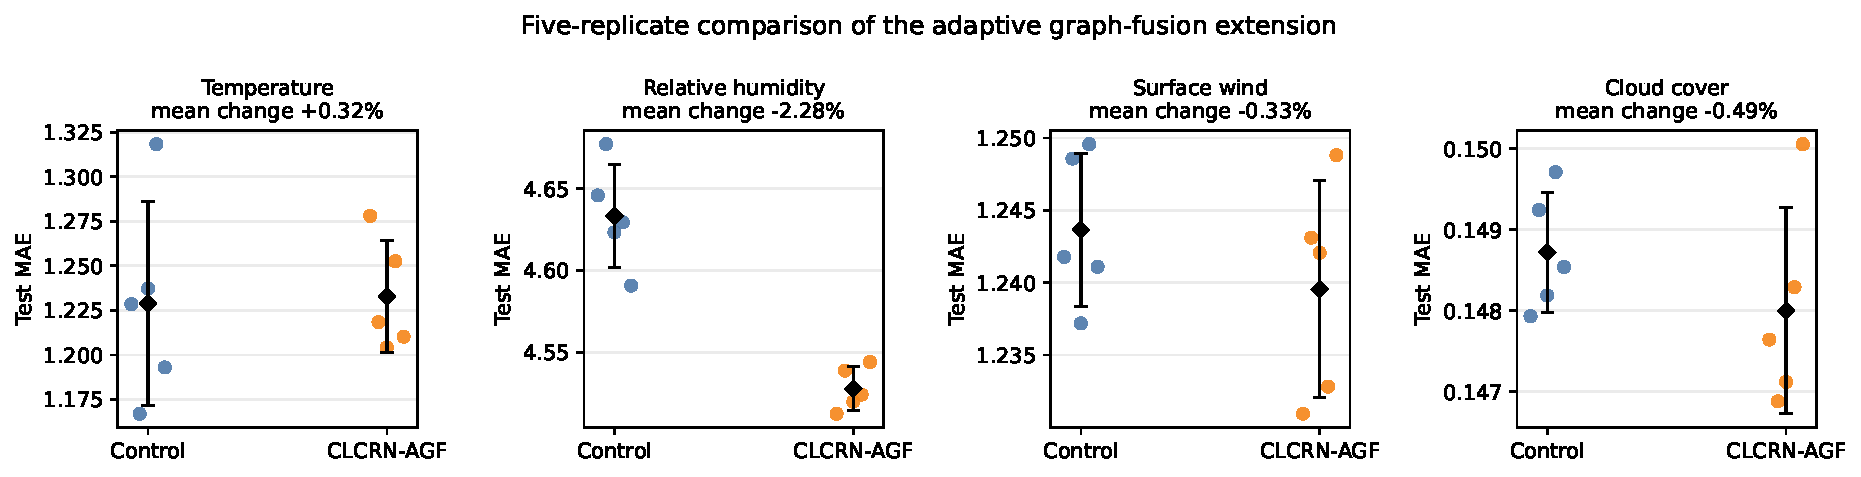
\includegraphics[width=\linewidth]{fig_primary_replicate_comparison.pdf}
\caption{\textbf{Test MAE for the schedule-matched control and CLCRN-AGF.}
Dots show individual seed replicates; diamonds show mean $\pm$ one standard
deviation. The humidity improvement is consistent across all five seed labels,
whereas the other tasks show overlapping or mixed changes.}
\label{fig:primary}
\end{figure}

\subsection*{Contextual benchmarks}
Table~\ref{tab:context} distinguishes results generated in this study from
external published values. Persistence is evaluated directly on the current
test split. ``Published CLCRN'' is copied from Lin et al.~\cite{lin2022conditional}
after restoring the humidity and cloud-cover reporting scales used by the
current evaluation code. ``Reproduced CLCRN'' is a single independent run of
the public implementation. The two final rows are five-seed results generated
under the revised schedule.

\begin{table}[htbp]
\caption{Contextual test results. Published CLCRN values are external
references, not newly generated results. Reproduced CLCRN is a single run;
control and CLCRN-AGF are five-seed means. Lower is better.}
\label{tab:context}
\centering
\scriptsize
\resizebox{\linewidth}{!}{%
\begin{tabular}{lrrrrrrrr}
\toprule
Method & \multicolumn{2}{c}{Temperature} & \multicolumn{2}{c}{Relative humidity}
& \multicolumn{2}{c}{Surface wind} & \multicolumn{2}{c}{Cloud cover}\\
\cmidrule(lr){2-3}\cmidrule(lr){4-5}\cmidrule(lr){6-7}\cmidrule(lr){8-9}
& MAE & RMSE & MAE & RMSE & MAE & RMSE & MAE & RMSE\\
\midrule
Persistence (current split) & 1.421 & 2.700 & 6.425 & 10.447 & 1.537 & 2.535 & 0.1620 & 0.2725\\
Published CLCRN~\cite{lin2022conditional} & 1.169 & 1.883 & 4.531 & 7.078 & 1.326 & 2.129 & 0.1491 & 0.2456\\
Reproduced CLCRN (one seed) & 1.192 & 2.246 & 4.677 & 7.309 & 1.384 & 2.266 & 0.1564 & 0.2574\\
Schedule-matched control (five seeds) & 1.229 & 2.097 & 4.633 & 7.237 & 1.244 & 1.977 & 0.1487 & 0.2473\\
CLCRN-AGF (five seeds) & 1.233 & 2.020 & 4.528 & 7.019 & 1.240 & 1.973 & 0.1480 & 0.2470\\
\bottomrule
\end{tabular}}
\end{table}

The contextual comparison shows why the extension should not be described as
uniformly superior. CLCRN-AGF improves on the published reference for
relative humidity and wind, is mixed for cloud cover, and does not improve
temperature. Differences
from the external reference also combine architecture, software environment,
and training-protocol effects; the schedule-matched control in
Table~\ref{tab:primary}
is therefore the primary causal comparison.

\subsection*{Component ablations}
The experiment archive also contains component ablations. Table~\ref{tab:ablation}
separates three kinds of evidence: 100-epoch, three-seed ablations for
temperature and relative humidity, and a 20-epoch single-seed screening run
over all four tasks. The full-budget humidity comparison uses seeds
2023--2025. The w/o gated fusion humidity completion was trained with
automatic mixed precision after repeated standard-precision runs exhausted
the local CUDA allocator; checkpoint selection and test evaluation still use
the same corrected zero-inclusive evaluator.

In the 100-epoch temperature ablation, removing the entire adaptive graph
branch worsens RMSE relative to the full model, while replacing the learned
gate by mean fusion gives similar or slightly lower mean errors. Thus the
gate is not uniformly beneficial for temperature. In the full-budget humidity
ablation, both adaptive-graph variants improve on the model without the
adaptive graph branch. The full gated model has the lowest mean MAE and RMSE,
but the mean-fusion variant remains close and was completed under the
mixed-precision caveat described above. We therefore treat this block as
sensitivity evidence that supports adaptive graph mixing, not as a definitive
precision-matched test of the gate. Figure~\ref{fig:ablation} visualizes the
two full-budget ablation blocks with seed-level points. The 20-epoch screening
run reaches the same qualitative warning: relative humidity is the most
sensitive task, whereas wind, temperature, and cloud-cover screening results
are mixed.

\begin{table}[htbp]
\caption{Component ablations. The first two blocks report 100-epoch
three-seed ablations at the full 12-hour horizon; the final block reports a
20-epoch single-seed screening ablation for all four tasks. Lower is better.}
\label{tab:ablation}
\centering
\scriptsize
\resizebox{\linewidth}{!}{%
\begin{tabular}{lllrr}
\toprule
Budget & Task & Variant & MAE & RMSE\\
\midrule
100 epochs, 3 seeds & Temperature & w/o adaptive graph & $1.265\pm0.046$ & $2.143\pm0.024$\\
                    &             & w/o gated fusion   & $1.189\pm0.098$ & $2.018\pm0.079$\\
                    &             & Full CLCRN-AGF     & $1.222\pm0.026$ & $2.032\pm0.062$\\
\midrule
100 epochs, 3 seeds & Relative humidity & w/o adaptive graph & $4.615\pm0.021$ & $7.223\pm0.043$\\
                    &             & w/o gated fusion   & $4.575\pm0.042$ & $7.077\pm0.076$\\
                    &             & Full CLCRN-AGF     & $4.529\pm0.013$ & $7.011\pm0.015$\\
\midrule
20 epochs, 1 seed & Temperature & w/o adaptive graph & 2.105 & 3.193\\
                  &             & w/o gated fusion   & 2.716 & 3.665\\
                  &             & Full CLCRN-AGF     & 2.356 & 3.273\\
                  & Relative humidity & w/o adaptive graph & 13.390 & 18.739\\
                  &             & w/o gated fusion   & 5.356 & 8.641\\
                  &             & Full CLCRN-AGF     & 5.151 & 8.097\\
                  & Surface wind & w/o adaptive graph & 1.371 & 2.199\\
                  &             & w/o gated fusion   & 1.542 & 2.478\\
                  &             & Full CLCRN-AGF     & 1.483 & 2.319\\
                  & Cloud cover & w/o adaptive graph & 0.1550 & 0.2511\\
                  &             & w/o gated fusion   & 0.1557 & 0.2551\\
                  &             & Full CLCRN-AGF     & 0.1559 & 0.2529\\
\bottomrule
\end{tabular}}
\vspace{2pt}

\parbox{\linewidth}{\scriptsize Values are mean$\pm$sample standard deviation
for the three-seed blocks. The humidity w/o gated fusion run used automatic
mixed precision for training; all reported test metrics use the same
zero-inclusive evaluator.}
\end{table}

\begin{figure}[htbp]
\centering
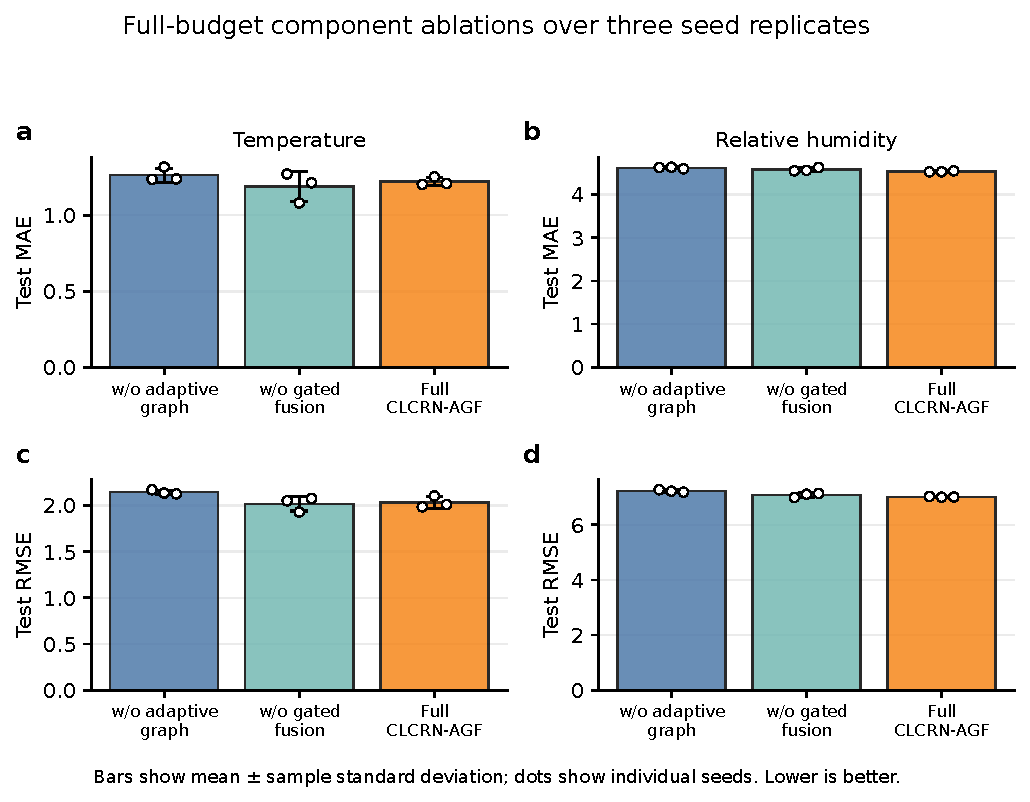
\includegraphics[width=0.96\linewidth]{fig_component_ablation_100ep.pdf}
\caption{\textbf{Full-budget component ablations for temperature and relative
humidity.} Bars show mean $\pm$ sample standard deviation across seeds
2023--2025, and dots show individual seed results. Panels a--b show test MAE;
panels c--d show test RMSE. The relative-humidity w/o gated fusion run used
automatic mixed precision during training; all reported test metrics use the
same zero-inclusive evaluator. Lower is better.}
\label{fig:ablation}
\end{figure}

\subsection*{Computational cost}
The AGF encoder approximately doubles the number of trainable parameters and
increases inference memory because it constructs a dense node-similarity
matrix before top-$k$ selection. Table~\ref{tab:efficiency} reports direct
measurements on the same NVIDIA GeForce RTX 5090 Laptop GPU. The extension is
compact relative to global foundation models, but it is not cost-free and is
not asymptotically linear in the number of nodes.

\begin{table}[htbp]
\caption{Measured model size and inference cost. Timings are milliseconds per
test batch; memory is peak allocated GPU memory during inference.}
\label{tab:efficiency}
\centering
\small
\begin{tabular}{llrrr}
\toprule
Task & Variant & Parameters & Inference (ms) & Memory (MB)\\
\midrule
Temperature & CLCRN & 39,268 & 202.6 & 352.3\\
            & CLCRN-AGF & 80,892 & 211.9 & 634.5\\
Relative humidity & CLCRN & 39,268 & 206.7 & 353.1\\
                  & CLCRN-AGF & 80,892 & 212.4 & 634.5\\
Surface wind & CLCRN & 39,437 & 197.3 & 368.6\\
             & CLCRN-AGF & 81,061 & 207.4 & 644.6\\
Cloud cover & CLCRN & 39,268 & 202.0 & 353.1\\
            & CLCRN-AGF & 80,892 & 203.4 & 634.5\\
\bottomrule
\end{tabular}
\end{table}

\subsection*{Gate diagnostics}
Gate values are summarized only as model diagnostics; their marginal
distribution does not by itself establish a physical interpretation. The
single-seed distributions in Figure~\ref{fig:gate} differ across tasks, but
causal attribution would require interventions on the two branches or
independent meteorological labels.

\begin{figure}[htbp]
\centering
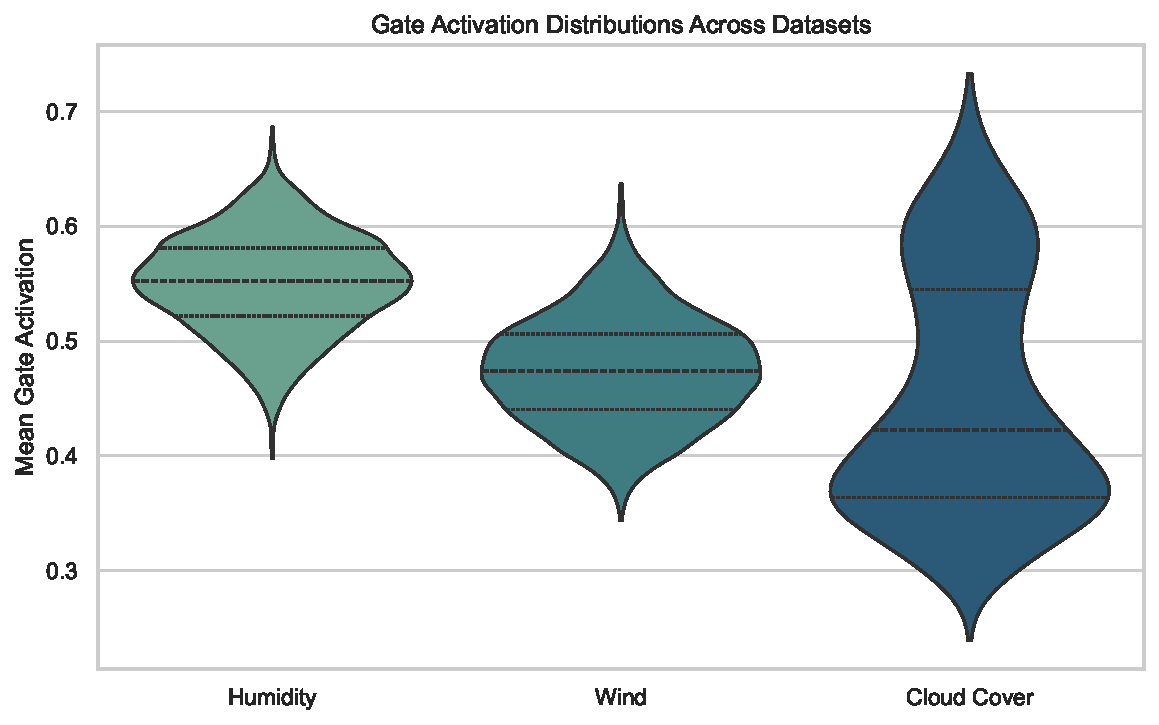
\includegraphics[width=0.82\linewidth]{fig_gate_distribution.pdf}
\caption{\textbf{Distribution of mean gate activations for three tasks in a
representative trained model.} The plot describes how the learned mixture
varies across samples. It should not be interpreted as proof that either
branch corresponds to a specific physical process.}
\label{fig:gate}
\end{figure}

\section*{Discussion}

The replicate experiment supports a narrow conclusion. Adding adaptive graph
fusion to CLCRN is beneficial for relative humidity under the tested setup:
the improvement is consistent across all five seed labels and the Welch
confidence interval excludes zero for both MAE and RMSE. For temperature,
wind, and cloud cover, the evidence does not support a general claim of
architectural superiority.

This task dependence is plausible but should not be over-interpreted.
Relative humidity may benefit from dependencies that are not captured by the
fixed local neighbourhood alone. The current experiment does not demonstrate
that the learned edges correspond to teleconnections or moisture corridors.
Establishing such a claim would require spatial edge analysis, comparisons
with meteorological indices, and perturbation tests.

The study also separates optimization effects from architectural effects.
The revised schedule substantially improves wind and cloud-cover results even
without AGF, while the additional AGF gain is small. Reporting only the best
single run would obscure this distinction. The five-replicate design is
therefore central to the present conclusions. The ablations further show that
the two AGF components do not contribute uniformly. For humidity, removing the
adaptive graph branch gives the weakest full-budget result, whereas mean
fusion without the learned gate remains close to the full model. For
temperature, mean fusion can also match or outperform the learned gate. The
evidence therefore supports the adaptive graph branch more strongly than it
supports a universal benefit from gated fusion, although the humidity gate
comparison should be interpreted cautiously because one ablation variant used
mixed-precision training.

Several limitations remain. First, the study inherits the compact
single-variable setup of the original CLCRN paper rather than evaluating
full-state medium-range weather prediction. Second, the current baseline set
contains persistence, the published CLCRN reference, and a schedule-matched
control; modern graph and non-graph baselines still need to be retrained under
the identical data and optimization pipeline. Third, the top-$k$ graph is
obtained from a dense $N\times N$ similarity matrix, giving quadratic
intermediate cost. Fourth, full-budget component ablations are now available
for temperature and relative humidity, but wind and cloud cover still rely on
the shorter 20-epoch component screening and should not be over-interpreted.
The humidity mean-fusion completion used mixed-precision training, so a fully
precision-matched ablation grid would be useful before making stronger claims
about the gate.

\section*{Conclusion}

This work evaluates an adaptive graph-fusion extension to the published
CLCRN weather-forecasting model. The revised manuscript distinguishes prior
CLCRN contributions, external published values, independent reproduction, and
new experiments. In five-replicate tests, CLCRN-AGF consistently improves
relative-humidity forecasting, while changes for temperature, wind, and cloud
cover are small or metric-dependent. The results therefore support adaptive
graph fusion as a task-dependent extension rather than a universally better
replacement for the original CLCRN encoder.

\section*{Methods}

\subsection*{Data and preprocessing}
We use the same four WeatherBench-derived tasks and public preprocessing
pipeline as the original CLCRN study~\cite{lin2022conditional}: 2-m
temperature (K), relative humidity (percentage points), 10-m surface wind
components ($u$ and $v$, m\,s$^{-1}$), and total cloud cover (fraction).
Hourly ERA5 records from 1 January 2010 through 31 December 2018 are mapped to
a $32\times64$ latitude--longitude grid with $N=2{,}048$ nodes.

Each example contains 12 consecutive hourly observations and targets the next
12 hours. Starting windows are sampled once per day (step size 24), producing
3,286 examples. The split is chronological and unshuffled: 2,300 training
examples (70\%), 329 validation examples (10\%), and 657 test examples
(20\%). Input and target variables are standardized with means and
standard deviations computed from the training subset only; metrics are
calculated after inverse transformation.

\subsection*{CLCRN backbone}
The backbone is the public CLCRN implementation of Lin et
al.~\cite{lin2022conditional}. CLConv generates a local kernel from each
centre-neighbour coordinate pair and multiplies it by geodesic-distance and
orientation factors. The resulting operator replaces linear transforms in a
graph-convolutional GRU and is used in a sequence-to-sequence
encoder--decoder. We retain this backbone without claiming its architecture
as a contribution of the present study.

\subsection*{Adaptive graph-fusion encoder}
Let $\mathbf{F}\in\R^{B\times T\times N\times d}$ be the concatenation of
the projected weather feature and the learned node embedding. Trainable
source and destination embeddings
$\mathbf{E}_{s},\mathbf{E}_{t}\in\R^{N\times d_e}$ define
\begin{equation}
\mathbf{A}=\operatorname{softmax}(\mathbf{E}_{s}\mathbf{E}_{t}^{\top}),
\end{equation}
where softmax is applied row-wise. For each node, the implementation retains
the self-edge and the $k-1$ largest remaining entries, then renormalizes the
selected weights. With neighbour set $\mathcal{T}_k(i)$,
\begin{equation}
\mathbf{m}_{i}=\sum_{j\in\mathcal{T}_k(i)}\tilde A_{ij}\mathbf{F}_{j}.
\end{equation}
Graph-mixed and residual features are projected separately:
\begin{equation}
\mathbf{q}_{i}=\mathbf{W}_{m}\mathbf{m}_{i}+\mathbf{b}_{m},\qquad
\mathbf{r}_{i}=\mathbf{W}_{r}\mathbf{F}_{i}+\mathbf{b}_{r}.
\end{equation}
The gated output is
\begin{align}
\mathbf{g}_{i}&=\sigma\!\left(\mathbf{W}_{g}
[\mathbf{r}_{i}\Vert\mathbf{q}_{i}]+\mathbf{b}_{g}\right),\\
\mathbf{z}_{i}&=\mathbf{g}_{i}\odot\mathbf{q}_{i}
+(1-\mathbf{g}_{i})\odot\mathbf{r}_{i}.
\end{align}
$\mathbf{z}$ is concatenated with the standard CLCRN encoder inputs before
the unchanged recurrent encoder. The control sets the AGF encoder off, so it
removes both adaptive mixing and its gate.

\subsection*{Training configuration}
Both variants use two recurrent layers, 32 hidden units, an 8-dimensional
weather-feature embedding, an 8-dimensional CLConv embedding, one CLConv
propagation view, and curriculum learning in the autoregressive decoder.
CLCRN-AGF uses 10-dimensional adaptive node embeddings, an 8-dimensional AGF
output, and $k=4$ selected neighbours including the self-edge. Training uses
Adam with learning rate 0.01, batch size 32, gradient-norm clipping at 5,
and a MultiStepLR schedule with milestones
$\{10,20,30,40,50\}$ and multiplicative factor 0.95. Models train for at
most 100 epochs and the checkpoint with the lowest validation MAE is used for
test evaluation.

Experiments were run with Python 3.13, PyTorch 2.10, CUDA 12.8, and an NVIDIA
GeForce RTX 5090 Laptop GPU. Seeds 2021--2025 are applied to NumPy and all
PyTorch random-number generators. We do not claim bitwise deterministic
reproducibility across hardware or library versions.
Primary control and CLCRN-AGF runs were trained in standard precision. The
additional relative-humidity w/o gated fusion ablation in
Table~\ref{tab:ablation} was completed with PyTorch automatic mixed precision
and batch size 32 because standard-precision attempts repeatedly failed with
CUDA allocator exhaustion on the available Windows GPU.

\subsection*{Metrics and statistical analysis}
MAE and RMSE are computed after inverse scaling. The corrected evaluator
includes all finite target values; zero is not treated as missing because zero
wind components and zero cloud cover are physically meaningful. Persistence
repeats the final input observation over the complete forecast horizon. The
primary analysis compares five seed replicates for each variant. For each
metric we report the mean and sample standard deviation across seeds, the mean
difference, a two-sided 95\% Welch confidence interval, and a two-sided Welch
test. All reported test rows use this zero-inclusive evaluator. For archived
runs with existing checkpoints, validation selection was recomputed with the
same corrected MAE among the saved checkpoints before test evaluation.

\subsection*{Computational complexity}
The original CLConv implementation materializes dense $N\times N$ kernel
operators, and AGF constructs a dense $N\times N$ similarity matrix before
top-$k$ selection. The implementation therefore has quadratic intermediate
memory and similarity-computation cost in $N$, despite sparse aggregation
after selection. Claims of linear scaling are not made.

\section*{Data availability}
The raw ERA5 variables are available through the
\href{https://github.com/pangeo-data/WeatherBench}{WeatherBench GitHub
repository} and the Copernicus Climate Data Store. The original CLCRN project
also provides preprocessed WeatherBench files through the data link described
in its public README. The preprocessing
period, variables, temporal windows, and chronological split used here are
specified in the Methods. Because the preprocessed arrays are derived from
third-party ERA5/WeatherBench data, they are not redistributed in the article
package. The submitted supplementary review archive contains the exact
configuration files, corrected metric tables, per-seed summaries, and scripts
needed to regenerate the reported tables and figures from the preprocessed
files.

\section*{Code availability}
The study uses the public CLCRN implementation, extended with the AGF module
and the corrected evaluation scripts described in this manuscript. The source
files, run configurations, corrected evaluation script, humidity
component-ablation completion script, and per-seed result summaries are
included in the supplementary software/review archive submitted with this
manuscript. The same materials are deposited in a public GitHub repository
(\href{https://github.com/gengx-prog/CLCRN-AGF-Scientific-Reports}{gengx-prog/CLCRN-AGF-Scientific-Reports}),
with the review archive attached to release
\href{https://github.com/gengx-prog/CLCRN-AGF-Scientific-Reports/releases/tag/v0.1-review}{v0.1-review}.


\FloatBarrier
\begin{thebibliography}{99}

\bibitem{bauer2015quiet}
  P.~Bauer, A.~Thorpe, and G.~Brunet.
  \newblock The quiet revolution of numerical weather prediction.
  \newblock \textit{Nature}, 525(7567):47--55, 2015.

\bibitem{rasp2020weatherbench}
  S.~Rasp, P.~D.~Dueben, S.~Scher, J.~A.~Weyn, S.~Mouatadid, and N.~Thuerey.
  \newblock WeatherBench: A benchmark data set for data-driven weather
    forecasting.
  \newblock \textit{J.\ Adv.\ Model.\ Earth Syst.},
    12(11):e2020MS002203, 2020.

\bibitem{pathak2022fourcastnet}
  J.~Pathak et al.
  \newblock {FourCastNet}: A global data-driven high-resolution weather model
    using adaptive {Fourier} neural operators.
  \newblock \textit{arXiv preprint arXiv:2202.11214}, 2022.

\bibitem{bi2023accurate}
  K.~Bi, L.~Xie, H.~Zhang, X.~Chen, X.~Gu, and Q.~Tian.
  \newblock Accurate medium-range global weather forecasting with 3D neural
    networks.
  \newblock \textit{Nature}, 619(7970):533--538, 2023.

\bibitem{lam2023learning}
  R.~Lam et al.
  \newblock Learning skillful medium-range global weather forecasting.
  \newblock \textit{Science}, 382(6677):1416--1421, 2023.

\bibitem{lin2022conditional}
  H.~Lin, Z.~Gao, Y.~Xu, L.~Wu, L.~Li, and S.~Z.~Li.
  \newblock Conditional local convolution for spatio-temporal meteorological
    forecasting.
  \newblock \textit{Proc.\ AAAI Conf.\ Artif.\ Intell.},
    36(7):7470--7478, 2022.
  \newblock doi:10.1609/aaai.v36i7.20711.

\bibitem{bai2020adaptive}
  L.~Bai, L.~Yao, C.~Li, X.~Wang, and C.~Wang.
  \newblock Adaptive graph convolutional recurrent network for traffic
    forecasting.
  \newblock In \textit{NeurIPS}, 2020.

\bibitem{wu2019graph}
  Z.~Wu, S.~Pan, G.~Long, J.~Jiang, and C.~Zhang.
  \newblock Graph WaveNet for deep spatial-temporal graph modeling.
  \newblock In \textit{IJCAI}, 2019.

\bibitem{wu2020connecting}
  Z.~Wu, S.~Pan, G.~Long, J.~Jiang, X.~Chang, and C.~Zhang.
  \newblock Connecting the dots: Multivariate time series forecasting with
    graph neural networks.
  \newblock In \textit{KDD}, 2020.

\bibitem{feng2022adaptive}
  A.~Feng and L.~Tassiulas.
  \newblock Adaptive graph spatial-temporal transformer network for traffic
  flow forecasting.
  \newblock \textit{arXiv preprint arXiv:2207.05064}, 2022.

\bibitem{huang2023adaptive}
  B.~Huang, H.~Dou, Y.~Luo, J.~Li, J.~Wang, and T.~Zhou.
  \newblock Adaptive spatiotemporal transformer graph network for traffic flow
    forecasting by {IoT} loop detectors.
  \newblock \textit{IEEE Internet of Things Journal},
    10(2):1642--1653, 2023.

\bibitem{cheon2026costefficient}
  M.~Cheon, J.-H.~Kim, Y.~Choi, Y.-H.~Choi, S.-Y.~Kang, J.-G.~Lee,
    Y.-G.~Ham, J.~Y.~Kim, and D.~Kang.
  \newblock Understanding machine learning weather prediction by designing a
    cost-efficient model with knowledge-oriented modules.
  \newblock \textit{Scientific Reports}, 16:2413, 2026.
  \newblock doi:10.1038/s41598-025-32366-3.

\bibitem{hu2025spherical}
  Y.~Hu, F.~Yin, W.~Zhang, K.~Ren, J.~Song, K.~Deng, and D.~Zhang.
  \newblock Spherical multigrid neural operator for improving autoregressive
    global weather forecasting.
  \newblock \textit{Scientific Reports}, 15:11522, 2025.
  \newblock doi:10.1038/s41598-025-96208-y.

\bibitem{frnda2022ecmwf}
  J.~Frnda, M.~Durica, J.~Rozhon, M.~Vojtekova, J.~Nedoma, and R.~Martinek.
  \newblock ECMWF short-term prediction accuracy improvement by deep learning.
  \newblock \textit{Scientific Reports}, 12:7898, 2022.
  \newblock doi:10.1038/s41598-022-11936-9.

\bibitem{alves2025spatiotemporal}
  D.~Alves, F.~Mendon\c{c}a, S.~S.~Mostafa, and F.~Morgado-Dias.
  \newblock A deep learning approach for improving spatiotemporal resolution
    of numerical weather prediction forecasts.
  \newblock \textit{Scientific Reports}, 15:32796, 2025.
  \newblock doi:10.1038/s41598-025-17867-5.

\bibitem{zanchi2023microclimate}
  M.~Zanchi, S.~Zapperi, and C.~A.~M.~La Porta.
  \newblock Harnessing deep learning to forecast local microclimate using
    global climate data.
  \newblock \textit{Scientific Reports}, 13:21062, 2023.
  \newblock doi:10.1038/s41598-023-48028-1.

\end{thebibliography}


\section*{Funding}
This research received no specific grant from any funding agency in the
public, commercial, or not-for-profit sectors.

\section*{Author contributions}
X.G. conceived the extension, implemented the software, conducted the
experiments and analysis, prepared the visualizations, and wrote the original
draft. H.-Y.L. supervised the study and reviewed and edited the manuscript.
Both authors reviewed and approved the final manuscript.

\section*{Competing interests}
The authors declare no competing interests.

\section*{Generative AI and AI-assisted technologies disclosure}
During preparation of this manuscript, the authors used AI-assisted language
editing to improve readability and organization. The authors reviewed and
edited all generated content and take full responsibility for the final
manuscript.

\end{document}
